\section{2D tunnel}

File: \texttt{03\_tunnel.yaml}

\subsection{Description}

The tutorial models the seepage site 23 m under the surface of the water
treatment plant tunnel Bedřichov in the granite rock massif. This
seepage site has fast reaction to the precipitation and measurements of
various chemical values are available.

The user will learn how to:

\begin{itemize}
\tightlist
\item
  Prescribe time-dependent input data.
\end{itemize}

The geometry consists of a rectangle 500 × 300 m with a circular hole of
diameter 3.6 m placed 23 meters under the surface, which represents a
plane perpendicular to the tunnel.

\subsection{Hydraulic model}

The hydraulic model was fitted on the shape of the flux field, where it
was assumed that the tunnel drains only a part of the model surface. In
particular, the model was fitted on the estimated discharge of the
seepage site.

We impose the following input data (see Figure \ref{fig:tunnel_geom}):

\begin{itemize}
\tightlist
\item
  The hydraulic conductivity of the rock medium is set to 2.59e-2 m/day
  (= 3e-7 m/s);
\item
  On the surface we prescribe the annual precipitation 2.33e-3 m/day (=
  852 mm/yr);
\item
  On the bottom part ``.base'' we prescribe the pressure 270 m because
  of assumption of local groundwater flow;
\item
  In the tunnel, the measured flux -9.16e-2 m/day (= -1.06e-6 m/s) is
  prescribed.
\end{itemize}

For convenience we use day as the unit of time. The corresponding YAML
code is:

\begin{verbatim}
input_fields:
  - region: rock
    conductivity: 2.59E-02
  - region: .tunnel
    bc_type: total_flux
    bc_flux: -9.16E-02
  - region: .base
    bc_type: dirichlet
    bc_pressure: 270
  - region: .surface
    bc_type: total_flux
    bc_flux: 2.33E-03
\end{verbatim}

\begin{figure}[htbp]
\centering
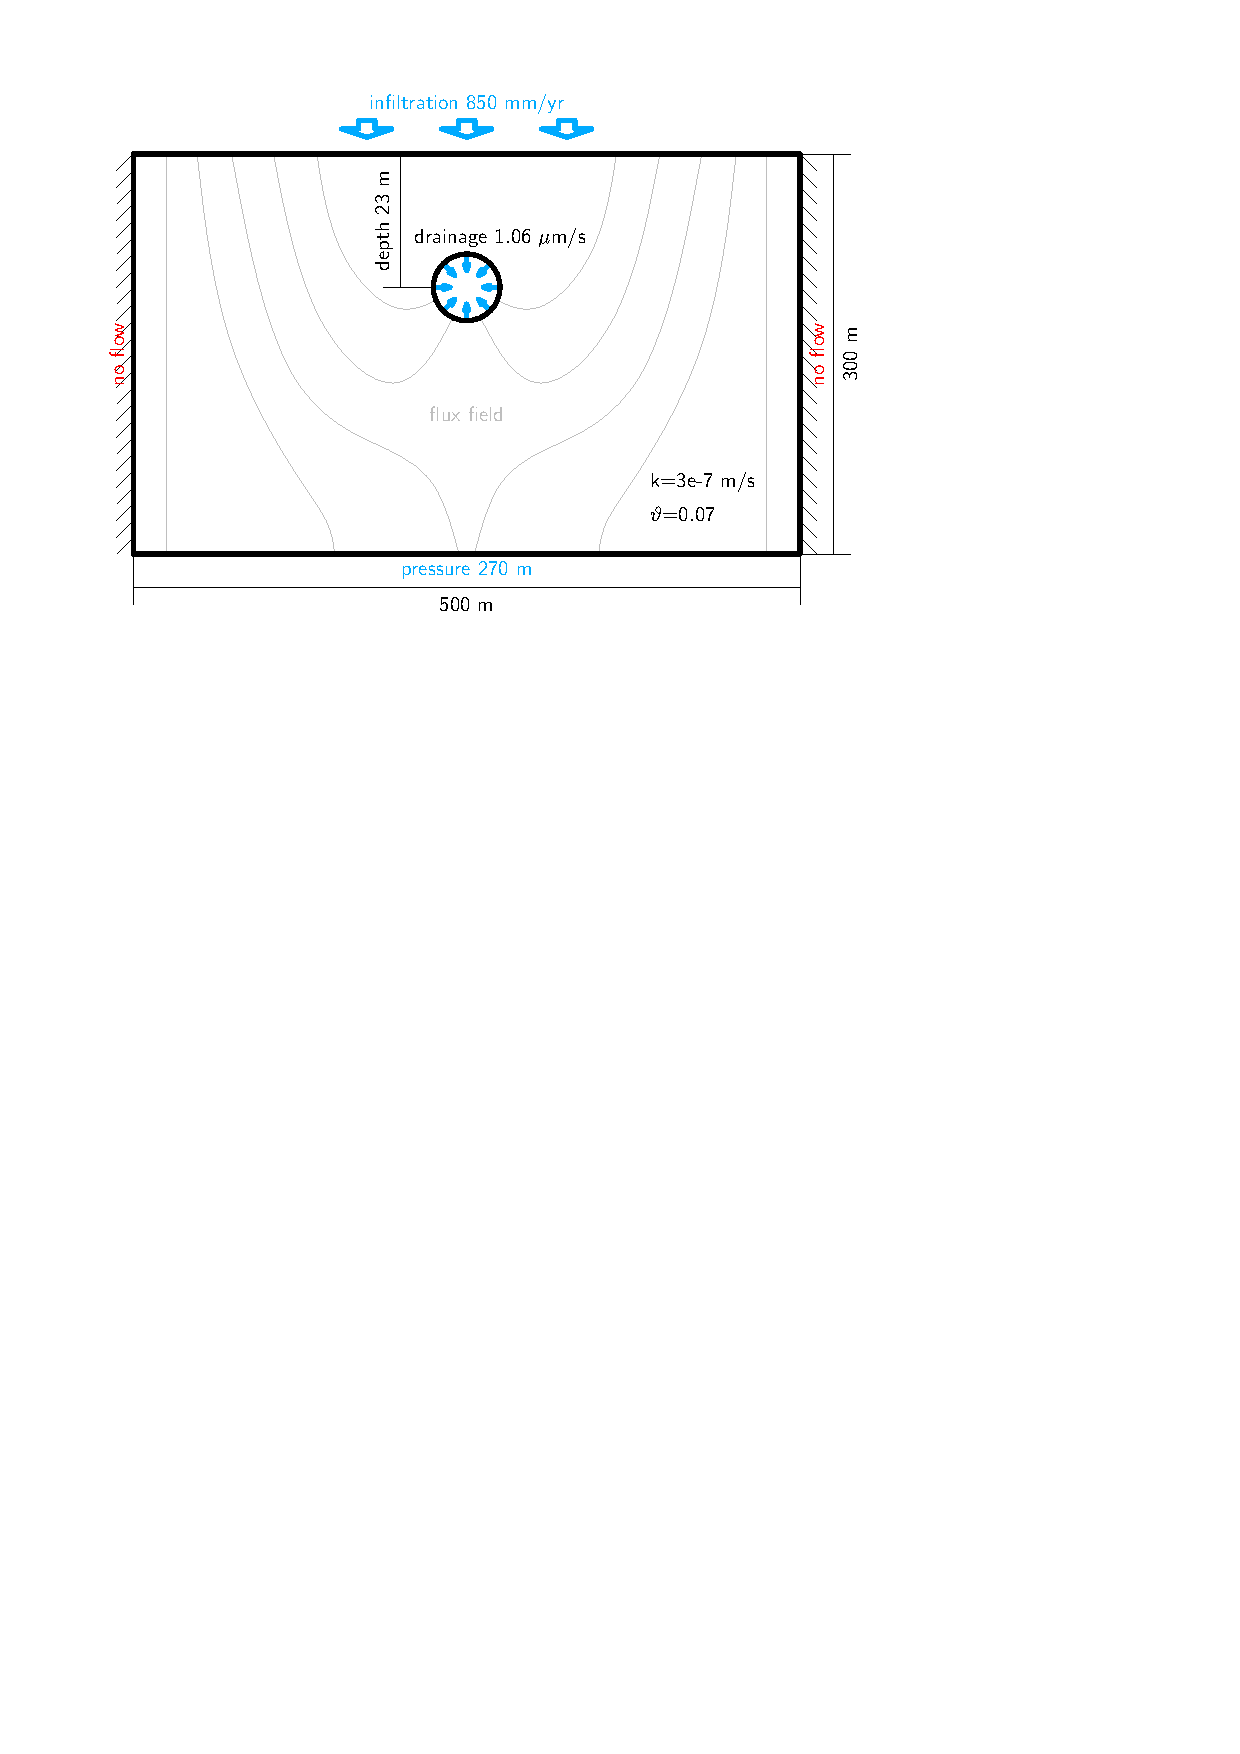
\includegraphics{tutor_figures/03_bc.pdf}
\caption{Geometry and boundary condition of
model.\label{fig:tunnel_geom}}
\end{figure}

The results are shown in Figure \ref{fig:flow}, where the flux field and
the pressure is shown. In the unsaturated layer the piezometric head is
depicted.

\begin{figure}[htbp]
\centering
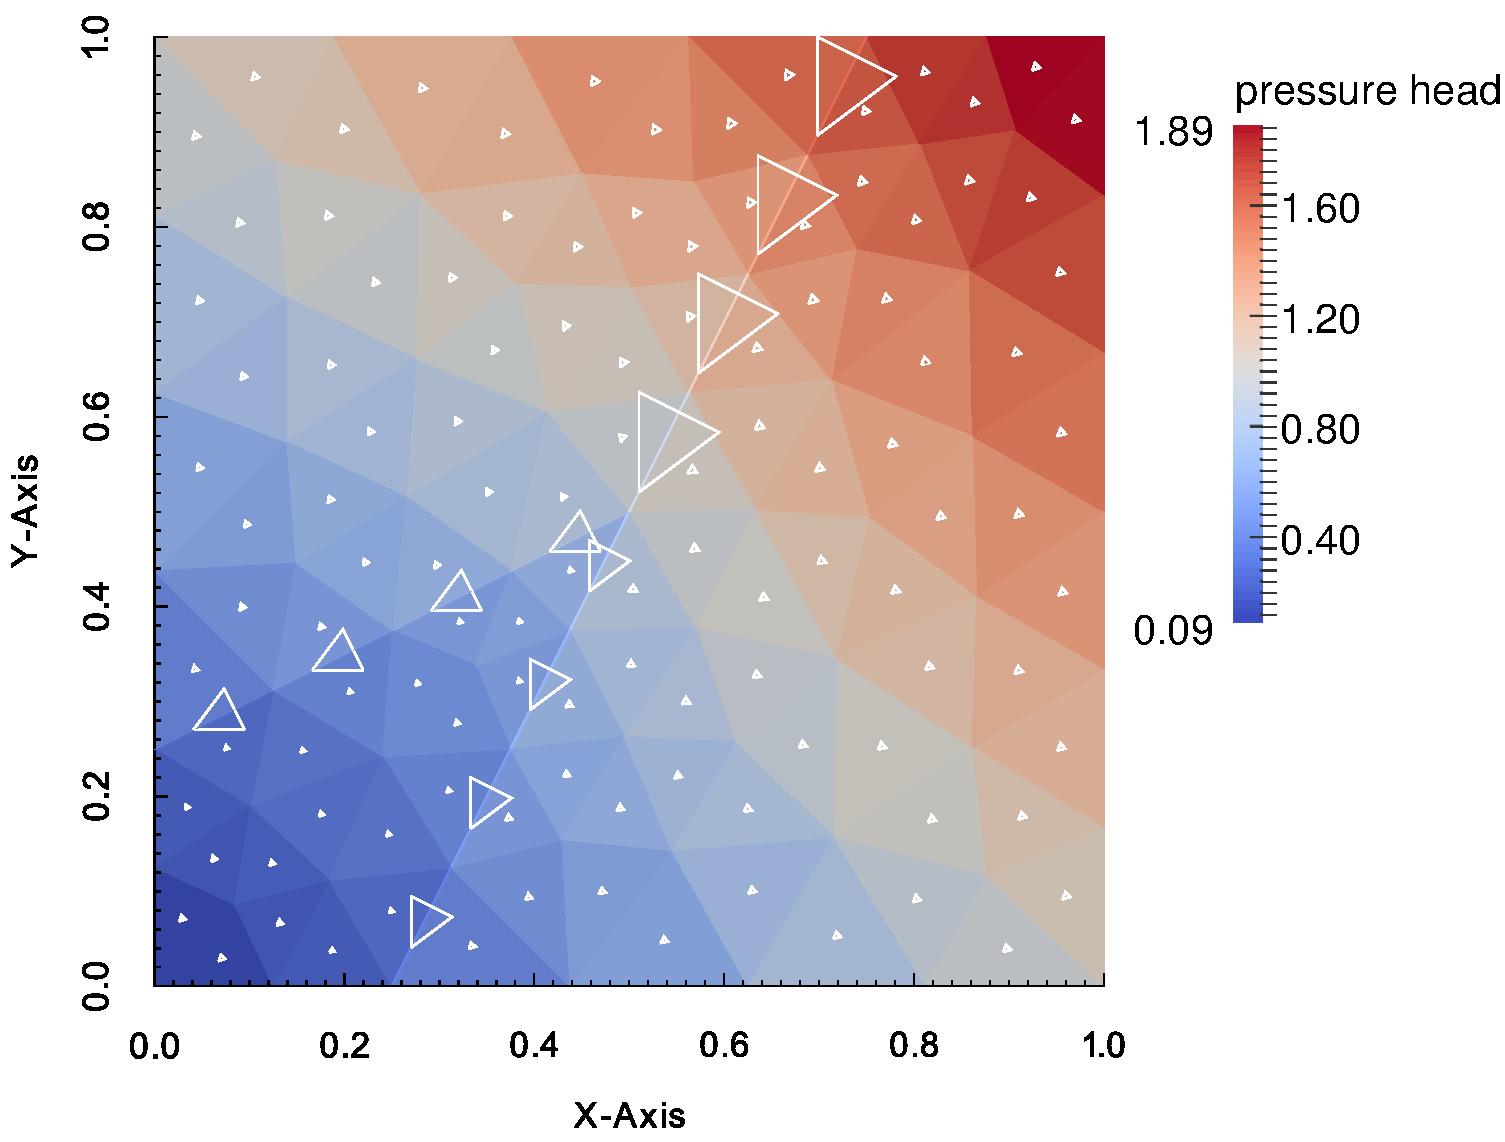
\includegraphics[width=1.00000\textwidth]{tutor_figures/03_flow.pdf}
\caption{Pressure, boundary of water level and piezometric head in
unsaturated zone and flux field.\label{fig:flow}}
\end{figure}

\subsection{Transport of real isotopes}

The stable isotope O-18 was sampled in monthly steps in precipitation at
nearby experimental catchment Uhlirska and at the seepage site 23m
depth. The measured values are used for the boundary condition on the
surface in the transport model as well as reference values in the
tunnel.

\subsubsection{Input}

We use the value 0.067 for porosity. The initial concentration of O-18
is set to -10.5 kg/m\textsuperscript{3}:

\begin{verbatim}
transport: !Solute_Advection_FV
  input_fields:
    - region: rock
      porosity: 0.067
      init_conc: -10.5
\end{verbatim}

The monthly measured values of \(\delta18\text{O}\) {[}per mil V-SMOW{]}
on the surface from the period 1/2006 till 6/2013 are supplied as the
boundary condition:

\begin{verbatim}
    - region: .surface
      bc_conc: -12.85443
      time: 11
    - region: .surface
      bc_conc: -14.00255
      time: 42
    - region: .surface
      bc_conc: -12.80081
      time: 72
    - region: .surface
      bc_conc: -12.34748
      time: 103
  ...
\end{verbatim}

\subsubsection{Results}

In Figure \ref{fig:conc_graph}, the computed mass flux through tunnel is
compared to the measured data. The evolution of the transported
substance is depicted in Figure \ref{fig:mass_real}.

\begin{figure}[htbp]
\centering
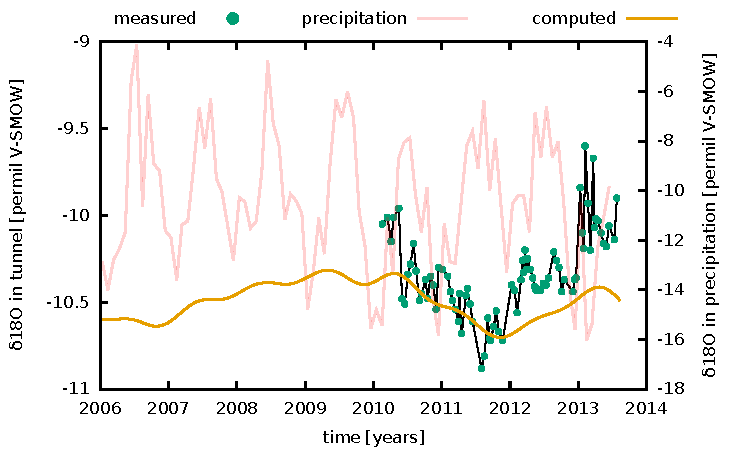
\includegraphics{tutor_figures/03_mass_flux.pdf}
\caption{Concentration of O-18 on the seepage site 23m under the
surface.\label{fig:conc_graph}}
\end{figure}

\begin{figure}[htbp]
\centering
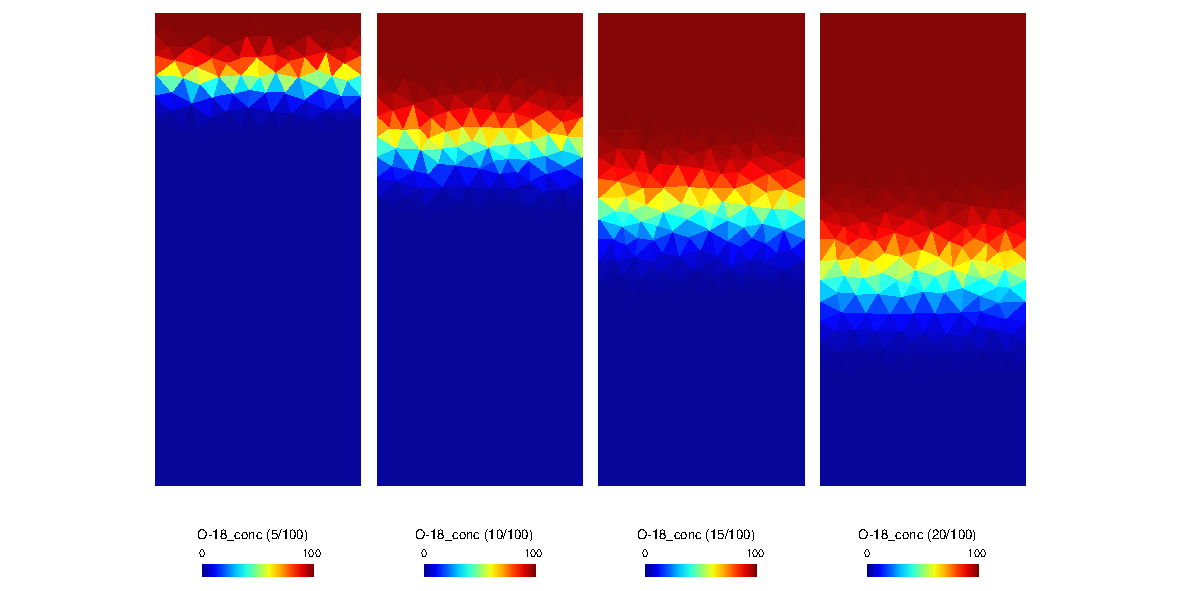
\includegraphics[width=1.00000\textwidth]{tutor_figures/03_transport.pdf}
\caption{Transport of isotopes in two-dimensional
model.\label{fig:mass_real}}
\end{figure}
